\section{Use Case 1: \\Benchmarking Safe Control Algorithms} \label{sec: usecase_benchmark}


To demonstrate SPARK’s capability as a benchmarking toolbox for safe control, we utilize it to systematically evaluate various algorithms under different constraints and objectives. By leveraging SPARK’s suite options, we ensure fair comparisons and gain insights into algorithmic performance, safety-efficiency trade-offs, and task complexity effects.  In our experiments, we aim to address the following questions:  

\textbf{Q1:}  
What are the overall benchmark results?  

\textbf{Q2:}  
How do various safe control algorithms balance the trade-off between safety and efficiency?  

\textbf{Q3:}  
How do different types of constraints affect algorithm performance?  

\textbf{Q4:}  
How does task complexity influence algorithm performance?  

\textbf{Q5:}  
How does the success rate of each algorithm compare?



\subsection{Experimental Setup}  
\paragraph{Experiment tasks}
By combining the robot, task, and constraint options introduced in \Cref{sec: suite_options}, $\textbf{8}$ benchmark tests are designed for the evaluation and comparison of algorithm performance. These predefined benchmark testing suites adhere to the standardized format: \texttt{\{Robot\}\_\{Task\}\_\{Constraint\}\_\{Version\}}. The configuration of all experiment tasks is introduced in \Cref{appendix: task_config}. In this format, \textbf{WG} represents \textit{Whole Body Goal}, \textbf{AG} stands for \textit{Arm Goal}, \textbf{SO} denotes \textit{Static Obstacle}, and \textbf{DO} refers to \textit{Dynamic Obstacle}. In particular, this benchmark does not provide WG as a standalone task; instead, WG indicates a combination of both \textit{Arm Goal} and \textit{Base Goal}. In addition to obstacles, self-collision is also taken into consideration. For more details, please refer to \Cref{appendix: self_collision}. In our experiments, we analyze and compare the performance of these algorithms using the metrics provided in \Cref{subsec:evaluation_metrics}.
We use $\sigma_{arm} = 0.002$, $\sigma_{base} = 0.05$, and $\sigma_{env} =\sigma_{self} = 0.0002$ to scale the scores to fit the magnitude of the raw distance. 



\paragraph{Comparison Group}  
To evaluate the performance of the \spark safe control library, we define a comparison group consisting of various alternative approaches. The methods in this group include all the techniques available in the safe control library \spark:
(i) Safe Set Algorithm (SSA)~\citep{liu2014control},  
(ii) Control Barrier Function (CBF)~\citep{ames2019control},  
(iii) Sublevel Safe Set (SSS)~\citep{wei2019safe},  
(iv) Potential Field Method (PFM)~\citep{khatib1986real}, and
(v) Sliding Mode Algorithm (SMA)~\citep{gracia2013reactive}.  



\paragraph{Overall Benchmark Results}
\Cref{tab:alg_metric_task} presents the overall benchmark performance results, evaluating different safety controllers in terms of safety and efficiency metrics. The experimental results indicate significant variations in the performance of different methods across various tasks and robotic setups. Specifically, in terms of motion accuracy and environmental safety, PFM exhibited the weakest overall performance, whereas optimization-based methods such as SSA, CBF, and SSS demonstrated a superior balance between safety and efficiency. Notably, despite not relying on optimization for safety control, SMA still managed to achieve a commendable trade-off between safety and efficiency.

PFM consistently showed low motion accuracy and environmental safety scores across all tasks, with particularly poor performance in fixed-base robotic tasks, where both its safety and execution efficiency were significantly lower than those of other methods. This suggests that PFM struggles to ensure feasibility in complex environments and is more susceptible to environmental constraints, leading to a higher risk of collisions. The primary issue with PFM is its reliance solely on repulsive forces in low-dimensional Cartesian space, making it ineffective in handling complex constraints in high-dimensional joint space, thereby limiting its safety control capabilities.

In contrast, SSA exhibited stable environmental safety across all tasks, demonstrating strong adaptability to external constraints. However, in fixed-base robotic tasks, SSA's motion accuracy was somewhat reduced, indicating that it may encounter challenges when dealing with scenarios where movement degrees of freedom are restricted.


CBF excelled in environmental safety, significantly outperforming PFM and showcasing its advantage in minimizing environmental collisions. However, compared to SSA, CBF exhibited slightly lower motion accuracy, suggesting that in certain tasks, it may sacrifice some execution efficiency to achieve higher safety.

As an optimization-based method, SSS demonstrated stable safety and execution efficiency across multiple tasks. For example, in some mobile robot tasks, its motion accuracy was comparable to SSA and CBF, while its environmental safety performance exceeded that of other methods. Additionally, in fixed-base robotic tasks, SSS achieved higher motion accuracy than other optimization methods, indicating that its optimization strategy effectively adapts to task requirements. 

Unlike optimization-based methods, SMA does not rely on optimization for safety control; instead, it refines control signals by decomposing the gradient of the safety index, thereby preserving effective task execution capabilities. The experimental results reveal that SMA generally achieved higher motion accuracy than other method in most tasks, while also maintaining high stability in environmental safety. This suggests that SMA can reduce environmental collision risks while ensuring smooth task execution.


% % \begin{figure*}[thbp]
%     \centering

%     % First row
%     \begin{subfigure}[b]{0.24\textwidth}
%         \includegraphics[width=\textwidth]{figure/conditional_success_matrix/G1FixedBase_DG_DO_v0_conditional_success_bar.pdf}
%         \caption{G1FixedBase\_DG\_DO}
%     \end{subfigure}
%     \begin{subfigure}[b]{0.24\textwidth}
%         \includegraphics[width=\textwidth]{figure/conditional_success_matrix/G1FixedBase_DG_SO_v0_conditional_success_bar.pdf}
%         \caption{G1FixedBase\_DG\_SO}
%     \end{subfigure}
%     \begin{subfigure}[b]{0.24\textwidth}
%         \includegraphics[width=\textwidth]{figure/conditional_success_matrix/G1FixedBase_SG_DO_v0_conditional_success_bar.pdf}
%         \caption{G1FixedBase\_SG\_DO}
%     \end{subfigure}
%     \begin{subfigure}[b]{0.24\textwidth}
%         \includegraphics[width=\textwidth]{figure/conditional_success_matrix/G1FixedBase_SG_SO_v0_conditional_success_bar.pdf}
%         \caption{G1FixedBase\_SG\_SO}
%     \end{subfigure}

%     % Second row
%     \begin{subfigure}[b]{0.24\textwidth}
%         \includegraphics[width=\textwidth]{figure/conditional_success_matrix/G1WholeBody_DG_DO_v0_conditional_success_bar.pdf}
%         \caption{G1WholeBody\_DG\_DO}
%     \end{subfigure}
%     \begin{subfigure}[b]{0.24\textwidth}
%         \includegraphics[width=\textwidth]{figure/conditional_success_matrix/G1WholeBody_DG_SO_v0_conditional_success_bar.pdf}
%         \caption{G1WholeBody\_DG\_SO}
%     \end{subfigure}
%     \begin{subfigure}[b]{0.24\textwidth}
%         \includegraphics[width=\textwidth]{figure/conditional_success_matrix/G1WholeBody_SG_DO_v0_conditional_success_bar.pdf}
%         \caption{G1WholeBody\_SG\_DO}
%     \end{subfigure}
%     \begin{subfigure}[b]{0.24\textwidth}
%         \includegraphics[width=\textwidth]{figure/conditional_success_matrix/G1WholeBody_SG_SO_v0_conditional_success_bar.pdf}
%         \caption{G1WholeBody\_SG\_SO}
%     \end{subfigure}

%     \caption{Conditional success plots for different tasks. The value at cell $(i, j)$ represents the proportion of environment settings successfully completed by the $i$-th algorithm that are also successfully completed by the $j$-th algorithm.}
%     \label{fig: conditional_success}
% \end{figure*}
% \begin{figure*}[htbp]
%     \centering
%     \vspace{2cm}  % Optional vertical space
%     \begin{tikzpicture}[transform canvas={xshift=-4.5cm}] 
%         % Define image size and spacing
%         \def\imgwidth{4.5cm}  % Image width
%         \def\xgap{4.5}  % X-axis spacing (horizontal)
%         \def\ygap{-4} % Y-axis spacing (vertical)
%         \def\xshift{-2} % Global X-axis shift for left movement

%         % First row (Row 1)
%         \node at (\xshift + 0, 0) {\includegraphics[width=\imgwidth]{figure/conditional_success_matrix/G1FixedBase_DG_DO_v0_conditional_success_bar.pdf}};
%         \node[below] at (\xshift + 0, -1.8) {\small (a) G1FixedBase\_DG\_DO};

%         \node at (\xshift + \xgap, 0) {\includegraphics[width=\imgwidth]{figure/conditional_success_matrix/G1FixedBase_DG_SO_v0_conditional_success_bar.pdf}};
%         \node[below] at (\xshift + \xgap, -1.8) {\small (b) G1FixedBase\_DG\_SO};

%         \node at (\xshift + 2*\xgap, 0) {\includegraphics[width=\imgwidth]{figure/conditional_success_matrix/G1FixedBase_SG_DO_v0_conditional_success_bar.pdf}};
%         \node[below] at (\xshift + 2*\xgap, -1.8) {\small (c) G1FixedBase\_SG\_DO};

%         \node at (\xshift + 3*\xgap, 0) {\includegraphics[width=\imgwidth]{figure/conditional_success_matrix/G1FixedBase_SG_SO_v0_conditional_success_bar.pdf}};
%         \node[below] at (\xshift + 3*\xgap, -1.8) {\small (d) G1FixedBase\_SG\_SO};

%         % Second row (Row 2)
%         \node at (\xshift + 0, \ygap) {\includegraphics[width=\imgwidth]{figure/conditional_success_matrix/G1WholeBody_DG_DO_v0_conditional_success_bar.pdf}};
%         \node[below] at (\xshift + 0, \ygap-1.8) {\small (e) G1WholeBody\_DG\_DO};

%         \node at (\xshift + \xgap, \ygap) {\includegraphics[width=\imgwidth]{figure/conditional_success_matrix/G1WholeBody_DG_SO_v0_conditional_success_bar.pdf}};
%         \node[below] at (\xshift + \xgap, \ygap-1.8) {\small (f) G1WholeBody\_DG\_SO};

%         \node at (\xshift + 2*\xgap, \ygap) {\includegraphics[width=\imgwidth]{figure/conditional_success_matrix/G1WholeBody_SG_DO_v0_conditional_success_bar.pdf}};
%         \node[below] at (\xshift + 2*\xgap, \ygap-1.8) {\small (g) G1WholeBody\_SG\_DO};

%         \node at (\xshift + 3*\xgap, \ygap) {\includegraphics[width=\imgwidth]{figure/conditional_success_matrix/G1WholeBody_SG_SO_v0_conditional_success_bar.pdf}};
%         \node[below] at (\xshift + 3*\xgap, \ygap-1.8) {\small (h) G1WholeBody\_SG\_SO};

%     \end{tikzpicture}
%     \vspace{6.3cm} 
    
%     \caption{Conditional success plots for different tasks. The value at cell $(i, j)$ represents the proportion of environment settings successfully completed by the $i$-th algorithm that are also successfully completed by the $j$-th algorithm.}
%     \label{fig: conditional_success}
% \end{figure*}


% \begin{figure*}[htbp]
% \centering

% \begin{subfigure}{0.24\linewidth}
%   \centering
%   \drawHeatMap{\dataA}
%   \caption{G1FixedBase\_DG\_DO}
% \end{subfigure}
% \hfill
% \begin{subfigure}{0.24\linewidth}
%   \centering
%   \drawHeatMap{\dataB}
%   \caption{G1FixedBase\_DG\_SO}
% \end{subfigure}
% \hfill
% \begin{subfigure}{0.24\linewidth}
%   \centering
%   \drawHeatMap{\dataC}
%   \caption{G1FixedBase\_SG\_DO}
% \end{subfigure}
% \hfill
% \begin{subfigure}{0.24\linewidth}
%   \centering
%   \drawHeatMap{\dataD}
%   \caption{G1FixedBase\_SG\_SO}
% \end{subfigure}

% \vspace{1em}
% \begin{subfigure}{0.24\linewidth}
%   \centering
%   \drawHeatMap{\dataE}
%   \caption{G1WholeBody\_DG\_DO}
% \end{subfigure}
% \hfill
% \begin{subfigure}{0.24\linewidth}
%   \centering
%   \drawHeatMap{\dataF}
%   \caption{G1WholeBody\_DG\_SO}
% \end{subfigure}
% \hfill
% \begin{subfigure}{0.24\linewidth}
%   \centering
%   \drawHeatMap{\dataG}
%   \caption{G1WholeBody\_SG\_DO}
% \end{subfigure}
% \hfill
% \begin{subfigure}{0.24\linewidth}
%   \centering
%   \drawHeatMap{\dataH}
%   \caption{G1WholeBody\_SG\_SO}
% \end{subfigure}

% \vspace{1em}
% \begin{tikzpicture}
%     \def\barWidth{8.0}
%     \def\barHeight{0.5}
%     \def\steps{50}

%     \foreach \s in {0,...,\steps} {
%         \pgfmathsetmacro{\f}{\s/\steps}  % fraction in [0..1]
%         \pgfmathparse{100*\f}            % colorValue = 0..100
%         \let\colorValue=\pgfmathresult

%         \pgfmathsetmacro{\xpos}{\f*\barWidth}

%         \fill[myPurple!\colorValue!yellow,draw=none]
%              (\xpos,0) rectangle
%              (\xpos + \barWidth/\steps, \barHeight);
%     }

%     \draw[black] (0,0) rectangle (\barWidth+0.15,\barHeight);

%     \node[below] at (0,0) {\footnotesize 0.4};
%     \node[below] at (\barWidth,0) {\footnotesize 1.0};

% \end{tikzpicture}

% \caption{Conditional success plots for different tasks. The value at cell $(i, j)$ represents the proportion of environment settings successfully completed by the $i$-th algorithm that are also successfully completed by the $j$-th algorithm.}
% \label{fig: conditional_success}
% \end{figure*}
\definecolor{myPurple}{rgb}{1.0, 0.0, 0.0}
\def\dataA{{
{1.0000, 0.5000, 0.5250, 0.9500, 0.9500},
{1.0000, 1.0000, 0.7500, 0.9500, 1.0000},
{0.9545, 0.6818, 1.0000, 0.9545, 0.9545},
{0.8085, 0.4043, 0.4468, 1.0000, 0.7872},
{0.9744, 0.5128, 0.5385, 0.9487, 1.0000}
}}

\def\dataB{{
{1.0000, 0.6977, 0.6279, 1.0000, 1.0000},
{0.9677, 1.0000, 0.7742, 0.9677, 0.9677},
{0.9643, 0.8571, 1.0000, 0.9643, 0.9643},
{0.9149, 0.6383, 0.5745, 1.0000, 0.9149},
{0.9773, 0.6818, 0.6136, 0.9773, 1.0000}
}}

\def\dataC{{
{1.0000, 0.4419, 0.7907, 0.9767, 1.0000},
{1.0000, 1.0000, 0.9474, 1.0000, 1.0000},
{1.0000, 0.5294, 1.0000, 0.9706, 1.0000},
{0.8750, 0.3958, 0.6875, 1.0000, 0.8958},
{0.9556, 0.4222, 0.7556, 0.9556, 1.0000}
}}

\def\dataD{{
{1.0000, 0.6200, 1.0000, 1.0000, 1.0000},
{1.0000, 1.0000, 1.0000, 1.0000, 1.0000},
{1.0000, 0.6200, 1.0000, 1.0000, 1.0000},
{1.0000, 0.6200, 1.0000, 1.0000, 1.0000},
{1.0000, 0.6200, 1.0000, 1.0000, 1.0000}
}}

\def\dataE{{
{1.0000, 0.6250, 0.9750, 0.5000, 0.9750},
{0.8621, 1.0000, 0.8966, 0.5862, 0.8966},
{0.8864, 0.5909, 1.0000, 0.4773, 0.9773},
{0.8696, 0.7391, 0.9130, 1.0000, 0.9130},
{0.8667, 0.5778, 0.9556, 0.4667, 1.0000}
}}

\def\dataF{{
{1.0000, 0.9592, 0.9184, 1.0000, 1.0000},
{0.9792, 1.0000, 0.9167, 0.9792, 1.0000},
{1.0000, 0.9778, 1.0000, 1.0000, 1.0000},
{1.0000, 0.9592, 0.9184, 1.0000, 1.0000},
{0.9800, 0.9600, 0.9000, 0.9800, 1.0000}
}}

\def\dataG{{
{1.0000, 0.5957, 0.9574, 0.6596, 0.9574},
{0.9333, 1.0000, 0.9333, 0.8000, 0.9333},
{0.9783, 0.6087, 1.0000, 0.6739, 1.0000},
{1.0000, 0.7742, 1.0000, 1.0000, 1.0000},
{0.9783, 0.6087, 1.0000, 0.6739, 1.0000}
}}

\def\dataH{{
{1.0000, 0.9592, 1.0000, 0.9796, 1.0000},
{1.0000, 1.0000, 1.0000, 1.0000, 1.0000},
{0.9800, 0.9400, 1.0000, 0.9600, 1.0000},
{1.0000, 0.9792, 1.0000, 1.0000, 1.0000},
{0.9800, 0.9400, 1.0000, 0.9600, 1.0000}
}}


% \newcommand{\rowLabel}[1]{%
%   \ifcase #1
%    \strut sss\or \strut sma\or \strut cbf\or \strut pfm\or \strut ssa%
%   \fi
% }
% \newcommand{\colLabel}[1]{%
%   \ifcase #1
%     \strut ssa\or \strut pfm\or \strut cbf\or \strut sma\or \strut sss%
%   \fi
% }

% \newcommand{\drawHeatMap}[1]{%
%     \begin{tikzpicture}[scale=0.7]
%     \pgfmathsetmacro{\rows}{5}
%     \pgfmathsetmacro{\cols}{5}
%     \def\data{#1}

%     \foreach \r in {1,...,\rows} {
%         \foreach \c in {1,...,\cols} {
%             \pgfmathparse{\data[\r-1][\c-1]}
%             \let\val=\pgfmathresult

%             \pgfmathparse{(\val - 0.85)/(1 - 0.85)*100}
%             \pgfmathsetmacro{\colorValue}{min(100,max(0,\pgfmathresult))}

%             \fill[
%               myPurple!\colorValue!yellow,
%               draw=black,
%               thin
%             ] (\c-1,\rows-\r) rectangle ++(1,1);
%         }
%     }
%     \draw[thick] (0,0) rectangle (\cols,\rows);

%     \foreach \r in {1,...,\rows} {
%         \pgfmathtruncatemacro{\idx}{\r-1} % \rows-\r=4..0
%         \node[left] at (-0.2,\r-0.5) {\small \rowLabel{\idx}};
%     }

%     \foreach \c in {1,...,\cols} {
%         \pgfmathtruncatemacro{\idx}{\c - 1} % 0..4
%         \node[above] at (\c-0.5,\rows+0.1) {\small \colLabel{\idx}};
%     }
%     \end{tikzpicture}%
% }

\begin{figure*}[htbp]
    \centering
    \vspace{2cm}  % Optional vertical space
    \begin{tikzpicture}[transform canvas={xshift=-4.5cm}] 
        % Define image size and spacing
        \def\imgwidth{4.5cm}  % Image width
        \def\xgap{4.5}  % X-axis spacing (horizontal)
        \def\ygap{-5} % Y-axis spacing (vertical)
        \def\xshift{-2} % Global X-axis shift for left movement

        % First row (Row 1)
        \node at (\xshift + 0, 0) {\drawHeatMap{\dataA}};
        \node[below] at (\xshift + 0, -2.4) {\small (a) G1FixedBase\_AG\_DO\_v0};

        \node at (\xshift + \xgap, 0) {\drawHeatMap{\dataB}};
        \node[below] at (\xshift + \xgap, -2.4) {\small (b) G1FixedBase\_AG\_DO\_v1};

        \node at (\xshift + 2*\xgap, 0) {\drawHeatMap{\dataC}};
        \node[below] at (\xshift + 2*\xgap, -2.4) {\small (c) G1FixedBase\_AG\_SO\_v0};

        \node at (\xshift + 3*\xgap, 0) {\drawHeatMap{\dataD}};
        \node[below] at (\xshift + 3*\xgap, -2.4) {\small (d) G1FixedBase\_AG\_SO\_v1};

        % Second row (Row 2)
        \node at (\xshift + 0, \ygap) {\drawHeatMap{\dataE}};
        \node[below] at (\xshift + 0, \ygap-2.4) {\small (e) G1WholeBody\_WG\_DO\_v0};

        \node at (\xshift + \xgap, \ygap) {\drawHeatMap{\dataF}};
        \node[below] at (\xshift + \xgap, \ygap-2.4) {\small (f) G1WholeBody\_WG\_DO\_v1};

        \node at (\xshift + 2*\xgap, \ygap) {\drawHeatMap{\dataG}};
        \node[below] at (\xshift + 2*\xgap, \ygap-2.4) {\small (g) G1WholeBody\_WG\_SO\_v0};

        \node at (\xshift + 3*\xgap, \ygap) {\drawHeatMap{\dataH}};
        \node[below] at (\xshift + 3*\xgap, \ygap-2.4) {\small (h) G1WholeBody\_WG\_SO\_v1};
        
        \def\barWidth{8.0}
        \def\barHeight{0.5}
        \def\steps{50}
    
        \foreach \s in {0,...,\steps} {
            \pgfmathsetmacro{\f}{\s/\steps}  % fraction in [0..1]
            \pgfmathparse{100*\f}            % colorValue = 0..100
            \let\colorValue=\pgfmathresult
    
            \pgfmathsetmacro{\xpos}{\f*\barWidth}
    
            \fill[myPurple!\colorValue!yellow,draw=none]
                 (\xpos, 1.75*\ygap) rectangle
                 (\xpos + \barWidth/\steps, \barHeight+ 1.75*\ygap);
        }
    
        \draw[black] (0, 1.75*\ygap) rectangle (\barWidth+0.15,\barHeight+ 1.75*\ygap);
    
        \node[below] at (0, 1.75*\ygap) {\footnotesize 0.85};
        \node[below] at (\barWidth, 1.75*\ygap) {\footnotesize 1.0};
    \end{tikzpicture}
    \vspace{9cm} 
    
    \caption{Conditional success plots for different tasks. The value at cell $(i, j)$ represents the proportion of environment settings successfully completed by the $i$-th algorithm that are also successfully completed by the $j$-th algorithm.}
    \label{fig: conditional_success}
\end{figure*}


\paragraph{Trade-off between Safety and Efficiency}


Balancing performance between safety and efficiency is a key challenge for every safe controller. To explore this trade-off, we tuned the parameters of each safe control algorithm across various scales: from 0 to 1 in steps of 0.1, from 1 to 10 in steps of 1, from 10 to 100 in steps of 10, and from 100 to 1000 in steps of 10. These experiments were conducted under different tasks, enabling us to plot safety and efficiency performance on the same graph. By extracting the convex hull of the sampled parameters,We generated the trade-off curves and selected two representative scenarios, as shown in \Cref{fig: param_tuning_subset}, which illustrate how each controller balances safety and efficiency.
The efficiency is defined as $\frac{J_{arm} + J_{base}}{2}$ and is plotted on the x-axis, while the average safety score ($\frac{M_{self}+ M_{env}}{2}$) is plotted along the y-axis.


\begin{figure}[htbp]
    \centering
    \begin{tikzpicture} 
        % Define image size and spacing
        \def\imgwidth{4cm}  % Image width
        \def\xgap{4.5}  % X-axis spacing

        % First image: G1FixedBase_SG_DO_v0
        \node at (0, 0) {\includegraphics[width=\imgwidth]{figure/param_tuning/G1FixedBase_SG_DO_v0_convex.pdf}};
        \node[below] at (0, -2) {\small (a) G1FixedBase\_AG\_DO\_v0};

        % Second image: G1WholeBody_SG_DO_v0 (shifted to the right)
        \node at (\xgap, 0) {\includegraphics[width=\imgwidth]{figure/param_tuning/G1WholeBody_SG_DO_v0_convex.pdf}};
        \node[below] at (\xgap, -2) {\small (b) G1WholeBody\_WG\_DO\_v0};

    \end{tikzpicture}

    \caption{Comparison of trade-off curves between safety and efficiency for different robot configurations.}
    \label{fig: param_tuning_subset}
\end{figure}

The results indicate that as parameters vary, safety and efficiency may adjust in opposition to each other. On average, SMA and PFM achieve better balance, while SSA, SSS and CBF excel at achieving higher safety scores without collisions. This behavior arises because, when their respective parameters \(c_{sma}\) and \(c_{pfm}\) approach zero, SMA and PFM cease correcting the reference control and revert to nominal controllers. However, PFM exhibits a less favorable trade-off curve compared to SMA due to its incompatibility with high-dimensional robotic systems and environments with multiple constraints.

Optimization-based methods, on the contrary, require their parameters to remain positive scalars, which consistently introduce additional safety constraints into the control problem. These methods prioritize ensuring safety over minimizing control deviations from the reference control. Unlike other optimization-based methods, CBF simultaneously impacts both safety and efficiency. This is due to its control law, which enforces that \(\dot{\phi}\) remains below an upper bound.

When the CBF parameter \(\lambda_{cbf}\) is too small, the robot may reduce the safety index unnecessarily even in safe environments, negatively impacting efficiency. Additionally, a small \(\lambda_{cbf}\) limits the safety constraints' ability to react rapidly in unsafe situations. Conversely, a large \(\lambda_{cbf}\) imposes overly strict safety constraints, even for minor safety violations, which can hinder efficiency.

In the other comparison experiments, the parameter for each algorithm is picked to achieve the best trade-off balancing. The optimal parameters for each algorithm and task are marked in \Cref{fig: param_tuning} and \Cref{appendix: hyperparameters} reports the parameters used for the rest experiments.


\paragraph{Impacts of Constraint Types}  


As shown in \Cref{fig: benchmark_performance_fixed}, obstacle motion and obstacle number both significantly impact algorithm performance. Dynamic obstacles introduce greater safety challenges compared to static ones. The radar charts illustrate that when obstacles are in motion, the corresponding \textbf{Arm Tracking Score} and \textbf{Environment Safety Score} tend to decrease. Furthermore, a comparison between v0 and v1 reveals that v1, which has fewer obstacles, achieves higher \textbf{Arm Tracking Score} and \textbf{Environment Safety Score}. This observation underscores the fact that a greater number of obstacles exerts a more pronounced negative impact on performance.

The other benchmark performance comparison is provided in \Cref{app: benchmark_performance_app} and \Cref{tab:alg_metric_task}.

% As shown in \Cref{fig: benchmark_performance_fixed} and the tables in \Cref{tb:task_scores}, dynamic obstacles pose greater safety challenges compared to static obstacles. The trade-off curves reveal that when obstacles are in motion, both fixed-base tasks and whole-body tasks experience a decrease in safety scores for optimization-based approaches.
\begin{figure}[htbp]
    \centering
    \begin{tikzpicture} 
        % Define image size and spacing
        \def\imgwidth{4cm}  % Image width
        \def\xgap{4.5}  % X-axis spacing (horizontal)
        \def\ygap{-3.5} % Y-axis spacing (vertical)

        % First row
        \node at (0, 0) {\includegraphics[width=\imgwidth]{figure/full_evaluation/G1WholeBody_SG_DO_v0_radar.pdf}};
        \node[below] at (-0.5, -1.5) {\small (a) G1WholeBody\_WG\_DO\_v0};

        \node at (\xgap, 0) {\includegraphics[width=\imgwidth]{figure/full_evaluation/G1WholeBody_SG_DO_v1_radar.pdf}};
        \node[below] at (\xgap-0.5, -1.5) {\small (b) G1WholeBody\_WG\_DO\_v1};

        % Second row
        \node at (0, \ygap) {\includegraphics[width=\imgwidth]{figure/full_evaluation/G1WholeBody_SG_SO_v0_radar.pdf}};
        \node[below] at (-0.5, \ygap-1.5) {\small (c) G1WholeBody\_WG\_SO\_v0};

        \node at (\xgap, \ygap) {\includegraphics[width=\imgwidth]{figure/full_evaluation/G1WholeBody_SG_SO_v1_radar.pdf}};
        \node[below] at (\xgap-0.5, \ygap-1.5) {\small (d) G1WholeBody\_WG\_SO\_v1};

    \end{tikzpicture}

    \caption{Performance comparison of the benchmark.}
    \label{fig: benchmark_performance_fixed}
\end{figure}
\paragraph{Influence of Task Difficulty}  
From \Cref{fig: param_tuning_subset}, it is evident that task difficulty significantly affects performance. For instance, when the robot is required to track both arm and base goals using whole-body movement, its performance is lower compared to tasks where a fixed base allows it to focus solely on arm goal tracking. This is because tracking the robot's base goal may require sacrificing arm goal tracking to avoid collisions and reach the base target.  



\paragraph{Success Rate across various Algorithms}
In addition to evaluating average step-wise performance, it is crucial to assess whether the safe controllers can successfully complete tasks trajectory-wise. A trajectory is defined to be successful if the robot reaches the goal without collisions within a maximum number of steps. In this evaluation, 50 feasible environment settings were generated and each algorithm was tested under these settings. The maximum number of steps was set to 200.  
% \begin{table}[h]
% \centering
% \captionsetup{width=0.5\textwidth}
% \caption{Success rate for Different Tasks and Algorithms}
% \label{tb:success_rate}
% \scalebox{0.95}{
% \begin{tabular}{c|ccccc}
% \toprule
% \textbf{Task Name} & \textbf{SSA} & \textbf{PFM} & \textbf{CBF} & \textbf{SMA} & \textbf{SSS} \\
% \midrule
% G1WholeBody\_SG\_SO & 0.8333 & 0.2667 & 0.5833 & 0.6667 & \textbf{0.9333} \\
% G1WholeBody\_SG\_DO & 0.6667 & 0.3500 & 0.7500 & 0.4833 & \textbf{0.9000} \\
% G1WholeBody\_DG\_SO & 0.8500 & 0.4667 & 0.6000 & 0.5833 & \textbf{0.9333} \\
% G1WholeBody\_DG\_DO & \textbf{0.8667} & 0.2500 & 0.8167 & 0.4667 & 0.8333 \\
% G1FixedBase\_SG\_SO & 0.8333 & 0.3833 & 0.7667 & \textbf{0.9833} & 0.9167 \\
% G1FixedBase\_SG\_DO & 0.9333 & 0.4333 & 0.3667 & \textbf{0.9500} & 0.9333 \\
% G1FixedBase\_DG\_SO & 0.8333 & 0.3667 & 0.7333 & \textbf{0.9833} & 0.8833 \\
% G1FixedBase\_DG\_DO & 0.9333 & 0.4500 & 0.4833 & \textbf{0.9833} & 0.9333 \\
% \bottomrule
% \end{tabular}
% }
% \label{tab: success_rate}
% \end{table}
% \begin{table}[h]
% \centering
% \captionsetup{width=0.5\textwidth}
% \caption{Success rate for Different Tasks and Algorithms}
% \label{tb:success_rate}
% \scalebox{0.95}{
% \begin{tabular}{c|ccccc}
% \toprule
% \textbf{Task Name} & \textbf{SSA} & \textbf{PFM} & \textbf{CBF} & \textbf{SMA} & \textbf{SSS} \\
% \midrule
% G1WholeBody\_SG\_SO & \textbf{0.9333} & 0.5667 & \textbf{0.9333} & 0.6333 & \textbf{0.9333} \\
% G1WholeBody\_SG\_DO & 0.7833 & 0.5667 & \textbf{0.8500} & 0.4667 & \textbf{0.8500} \\
% G1WholeBody\_DG\_SO & 0.9000 & 0.5333 & 0.9167 & 0.6000 & \textbf{0.9500} \\
% G1WholeBody\_DG\_DO & 0.7667 & 0.6333 & \textbf{0.8500} & 0.4167 & 0.8333 \\
% G1FixedBase\_SG\_SO & 0.8667 & 0.4167 & 0.7000 & \textbf{0.9500} & 0.9000 \\
% G1FixedBase\_SG\_DO & 0.8167 & 0.4167 & 0.4833 & \textbf{0.9500} & 0.8000 \\
% G1FixedBase\_DG\_SO & 0.9167 & 0.4333 & 0.7167 & 0.9000 & \textbf{0.9333} \\
% G1FixedBase\_DG\_DO & 0.8000 & 0.3500 & 0.4667 & \textbf{0.9333} & 0.8000 \\
% \bottomrule
% \end{tabular}
% }
% \label{tab: success_rate}
% \end{table}
\begin{table}[h]
\centering
\captionsetup{width=0.5\textwidth}
\caption{Success rate for Different Tasks and Algorithms}
\label{tb:success_rate}
\scalebox{0.9}{
\begin{tabular}{c|ccccc}
\toprule
\textbf{Task Name} & \textbf{SSA} & \textbf{PFM} & \textbf{CBF} & \textbf{SMA} & \textbf{SSS} \\
\midrule
G1WholeBody\_WG\_SO\_v1 & 0.9667 & 0.9500 & \textbf{1.0000} & 0.9667 & \textbf{1.0000} \\
G1WholeBody\_WG\_SO\_v0 & \textbf{0.9333} & 0.5667 & \textbf{0.9333} & 0.6333 & \textbf{0.9333} \\
G1WholeBody\_WG\_DO\_v1 & 0.9833 & 0.9500 & 0.8833 & 0.9833 &  \textbf{1.0000} \\
G1WholeBody\_WG\_DO\_v0 & 0.7833 & 0.5667 & \textbf{0.8500} & 0.4667 & \textbf{0.8500} \\
G1FixedBase\_AG\_SO\_v1 &  \textbf{1.0000}& 0.6667 &  \textbf{1.0000}& \textbf{1.0000} &\textbf{1.0000} \\
G1FixedBase\_AG\_SO\_v0 & 0.8667 & 0.4167 & 0.7000 & \textbf{0.9500} & 0.9000 \\
G1FixedBase\_AG\_DO\_v1 & 0.8833 & 0.6333 & 0.5500 & \textbf{0.9500} & 0.9000 \\
G1FixedBase\_AG\_DO\_v0 & 0.8167 & 0.4167 & 0.4833 & \textbf{0.9500} & 0.8000 \\
\bottomrule
\end{tabular}
}
\label{tab: success_rate}
\end{table}

The success results of each algorithm are listed in \Cref{tab: success_rate}, which shows the conditional success rate of the algorithms. Detailed results are provided in \Cref{appendix: success_rate}. From these results, it can be observed that SSS achieves the highest success rate for tasks involving whole-body motion, The second is CBF. For tasks with a fixed base, SMA attains the highest success rate, while SSS and SSA also perform well. This suggests that optimization-based methods, such as SSS and SSA, are better equipped to handle multiple constraints in complex environments. Conversely, SMA's safe correction is more efficient for relatively simple tasks. Among all algorithms, PFM exhibits the lowest success rate. 

\definecolor{myPurple}{rgb}{1.0, 0.0, 0.0}
\def\dataA{{
{1.0000, 0.5000, 0.5250, 0.9500, 0.9500},
{1.0000, 1.0000, 0.7500, 0.9500, 1.0000},
{0.9545, 0.6818, 1.0000, 0.9545, 0.9545},
{0.8085, 0.4043, 0.4468, 1.0000, 0.7872},
{0.9744, 0.5128, 0.5385, 0.9487, 1.0000}
}}

\def\dataB{{
{1.0000, 0.6977, 0.6279, 1.0000, 1.0000},
{0.9677, 1.0000, 0.7742, 0.9677, 0.9677},
{0.9643, 0.8571, 1.0000, 0.9643, 0.9643},
{0.9149, 0.6383, 0.5745, 1.0000, 0.9149},
{0.9773, 0.6818, 0.6136, 0.9773, 1.0000}
}}

\def\dataC{{
{1.0000, 0.4419, 0.7907, 0.9767, 1.0000},
{1.0000, 1.0000, 0.9474, 1.0000, 1.0000},
{1.0000, 0.5294, 1.0000, 0.9706, 1.0000},
{0.8750, 0.3958, 0.6875, 1.0000, 0.8958},
{0.9556, 0.4222, 0.7556, 0.9556, 1.0000}
}}

\def\dataD{{
{1.0000, 0.6200, 1.0000, 1.0000, 1.0000},
{1.0000, 1.0000, 1.0000, 1.0000, 1.0000},
{1.0000, 0.6200, 1.0000, 1.0000, 1.0000},
{1.0000, 0.6200, 1.0000, 1.0000, 1.0000},
{1.0000, 0.6200, 1.0000, 1.0000, 1.0000}
}}

\def\dataE{{
{1.0000, 0.6250, 0.9750, 0.5000, 0.9750},
{0.8621, 1.0000, 0.8966, 0.5862, 0.8966},
{0.8864, 0.5909, 1.0000, 0.4773, 0.9773},
{0.8696, 0.7391, 0.9130, 1.0000, 0.9130},
{0.8667, 0.5778, 0.9556, 0.4667, 1.0000}
}}

\def\dataF{{
{1.0000, 0.9592, 0.9184, 1.0000, 1.0000},
{0.9792, 1.0000, 0.9167, 0.9792, 1.0000},
{1.0000, 0.9778, 1.0000, 1.0000, 1.0000},
{1.0000, 0.9592, 0.9184, 1.0000, 1.0000},
{0.9800, 0.9600, 0.9000, 0.9800, 1.0000}
}}

\def\dataG{{
{1.0000, 0.5957, 0.9574, 0.6596, 0.9574},
{0.9333, 1.0000, 0.9333, 0.8000, 0.9333},
{0.9783, 0.6087, 1.0000, 0.6739, 1.0000},
{1.0000, 0.7742, 1.0000, 1.0000, 1.0000},
{0.9783, 0.6087, 1.0000, 0.6739, 1.0000}
}}

\def\dataH{{
{1.0000, 0.9592, 1.0000, 0.9796, 1.0000},
{1.0000, 1.0000, 1.0000, 1.0000, 1.0000},
{0.9800, 0.9400, 1.0000, 0.9600, 1.0000},
{1.0000, 0.9792, 1.0000, 1.0000, 1.0000},
{0.9800, 0.9400, 1.0000, 0.9600, 1.0000}
}}


\newcommand{\rowLabel}[1]{%
  \ifcase #1
   \strut SSS\or \strut SMA\or \strut CBF\or \strut PFM\or \strut SSA%
  \fi
}
\newcommand{\colLabel}[1]{%
  \ifcase #1
    \strut SSA\or \strut PFM\or \strut CBF\or \strut SMA\or \strut SSS%
  \fi
}


\newcommand{\drawHeatMap}[1]{%
    \begin{tikzpicture}[scale=0.6]
    \pgfmathsetmacro{\rows}{5}
    \pgfmathsetmacro{\cols}{5}
    \def\data{#1}

    \foreach \r in {1,...,\rows} {
        \foreach \c in {1,...,\cols} {
            \pgfmathparse{\data[\r-1][\c-1]}
            \let\val=\pgfmathresult

            \pgfmathparse{(\val - 0.85)/(1 - 0.85)*100}
            \pgfmathsetmacro{\colorValue}{min(100,max(0,\pgfmathresult))}

            \fill[
              myPurple!\colorValue!yellow,
              draw=black,
              thin
            ] (\c-1,\rows-\r) rectangle ++(1,1);
        }
    }
    \draw[thick] (0,0) rectangle (\cols,\rows);

    \foreach \r in {1,...,\rows} {
        \pgfmathtruncatemacro{\idx}{\r-1} % \rows-\r=4..0
        \node[left] at (-0.2,\r-0.5) {\scriptsize  \rowLabel{\idx}};
    }

    \foreach \c in {1,...,\cols} {
        \pgfmathtruncatemacro{\idx}{\c - 1} % 0..4
        \node[above] at (\c-0.5,\rows+0.1) {\scriptsize  \colLabel{\idx}};
    }
    \end{tikzpicture}%
}
\begin{figure}[htbp]
    \centering
    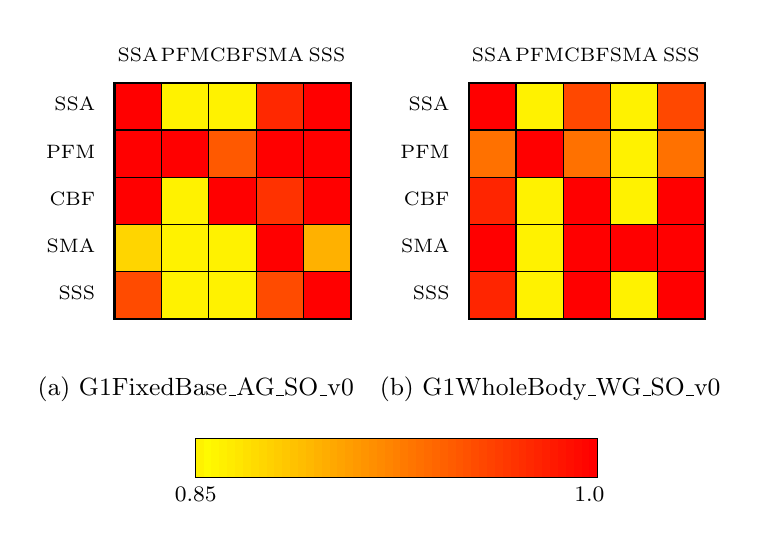
\begin{tikzpicture} 
        % Define image size and spacing
        \def\imgwidth{3cm}  % Image width
        \def\xgap{4.5}  % X-axis spacing (horizontal)
        \def\ygap{-2.3} % Y-axis spacing (vertical)

        % First heatmap
        \node at (0, 0) {\drawHeatMap{\dataC}};
        \node[below] at (0, -2.4) {\small (a) G1FixedBase\_AG\_SO\_v0};

        % Second heatmap
        \node at (\xgap, 0) {\drawHeatMap{\dataG}};
        \node[below] at (\xgap, -2.4) {\small (b) G1WholeBody\_WG\_SO\_v0};
        
        % Color bar
        \def\barWidth{5.0}
        \def\barHeight{0.5}
        \def\steps{50}
    
        \foreach \s in {0,...,\steps} {
            \pgfmathsetmacro{\f}{\s/\steps}  % fraction in [0..1]
            \pgfmathparse{100*\f}            % colorValue = 0..100
            \let\colorValue=\pgfmathresult
    
            \pgfmathsetmacro{\xpos}{\f*\barWidth}
    
            \fill[myPurple!\colorValue!yellow,draw=none]
                 (\xpos, \ygap-1.5) rectangle
                 (\xpos + \barWidth/\steps, \barHeight+\ygap-1.5);
        }
    
        \draw[black] (0, \ygap-1.5) rectangle (\barWidth+0.1,\barHeight+\ygap-1.5);
    
        \node[below] at (0, \ygap-1.5) {\footnotesize 0.85};
        \node[below] at (\barWidth, \ygap-1.5) {\footnotesize 1.0};
    \end{tikzpicture}

    \caption{Conditional success plots for selected tasks.}
    \label{fig: conditional_success_selected}
\end{figure}

Beyond individual success rates, it is also informative to examine the relative advantages between pairs of safe control algorithms. To do this, we define the conditional success rate \( P(B|A) \) as:
\begin{align}
    P(B|A) = \frac{\#(A \cap B)}{\#A}, \\ \nonumber
\end{align}
where \( \#(B \cap A) \) represents the number of environments successfully completed by both algorithm \( A \) and algorithm \( B \), and \( \#A \) represents the number of environments successfully completed only by algorithm \( A \).  

\Cref{fig: conditional_success_selected} presents a heatmap of the conditional success rates for each task where the value of the cell $(i, j)$ is calculated by $P(algo[j]|algo[i])$. The results indicate that optimization-based methods, such as SSA, SSS, and CBF, significantly outperform PFM and SMA in success rates. Furthermore, the comparison of conditional success rates reveals that \( P(\text{SSA}|\text{CBF}) > P(\text{CBF}|\text{SSA}) \) in five out of eight tasks, indicating that SSA successfully completes most of the trajectories that CBF can achieve in these cases. In contrast, CBF does not achieve the same success rate. Detailed conditional success rates are reported in \Cref{appendix: conditional_success_rate} and \Cref{app: conditional_success_app}.

In conclusion, using \spark as a safe control benchmark highlights its composability by enabling the convenient generation of large-scale testing configurations. As a benchmarking framework, it also provides users with a structured parameter-tuning process and a comprehensive understanding of the implemented safe control algorithms, aiding in the synthesis of the most suitable safe controller for each task. The results indicate that there is still significant room for improvement in safe controller design to achieve a fully guaranteed $100\%$ safety assurance, presenting further challenges for future research.